\documentclass[usenames,dvipsnames]{beamer}
\usepackage{tikz}
\usepackage{filecontents}
\usepackage[
    citestyle=numeric,  % Your citation style.
    bibstyle=numeric,         % Style for bibliography list. It will be numeric.
    sorting=none,             % The citations will be listed in the order of appearance
    backend=biber             % This is not necessary for newer versions of biblatex as
                              % it is the default, but it certainly helps to keep things
                              % explicit.
]{biblatex}
%\addbibresource{Bibliography/references}
\setbeamertemplate{bibliography item}{\insertbiblabel}
\addbibresource{\jobname.bib}
\begin{filecontents}{\jobname.bib}

@Article{journals/corr/PengSLMW16,
  title =	"Recent Advances in Cloud Radio Access Networks: System
		 Architectures, Key Techniques, and Open Issues",
  author =	"Mugen Peng and Yaohua Sun and Xuelong Li and Zhendong
		 Mao and Chonggang Wang",
  journal =	"CoRR",
  year = 	"2016",
  volume =	"abs/1604.00607",
  bibdate =	"2017-06-07",
  bibsource =	"DBLP,
		 http://dblp.uni-trier.de/db/journals/corr/corr1604.html#PengSLMW16",
  URL =  	"http://arxiv.org/abs/1604.00607",
}


@Article{journals/twc/TangTQ15,
  title =	"Cross-Layer Resource Allocation With Elastic Service
		 Scaling in Cloud Radio Access Network",
  author =	"Jianhua Tang and Wee-Peng Tay and Tony Q. S. Quek",
  journal =	"IEEE Trans. Wireless Communications",
  year = 	"2015",
  number =	"9",
  volume =	"14",
  bibdate =	"2017-06-09",
  bibsource =	"DBLP,
		 http://dblp.uni-trier.de/https://doi.org/10.1109/TWC.2015.2432023;
		 DBLP,
		 http://dblp.uni-trier.de/db/journals/twc/twc14.html#TangTQ15",
  pages =	"5068--5081",
}


@InProceedings{conf/wiopt/AlabbasiC17,
  title =	"Delay-aware green hybrid CRAN",
  author =	"Abdulrahman Alabbasi and Cicek Cavdar",
  publisher =	"IEEE",
  year = 	"2017",
  bibdate =	"2017-07-06",
  bibsource =	"DBLP,
		 http://dblp.uni-trier.de/https://doi.org/10.23919/WIOPT.2017.7959942;
		 DBLP,
		 http://dblp.uni-trier.de/db/conf/wiopt/wiopt2017.html#AlabbasiC17",
  booktitle =	"WiOpt",
  crossref =	"conf/wiopt/2017",
  ISBN = 	"978-3-9018-8290-6",
  pages =	"1--7",
  URL =  	"http://ieeexplore.ieee.org/xpl/mostRecentIssue.jsp?punumber=7951216",
}
@misc{wiki:C-RAN,
   author = "Wikipedia",
   title = "{C-RAN} --- {W}ikipedia{,} The Free Encyclopedia",
   year = "2018",
   howpublished = {\url{http://en.wikipedia.org/w/index.php?title=C-RAN&oldid=827881004}},
   note = "[Online; accessed 26-March-2018]"
 }
\end{filecontents}
\usetheme{Madrid}


\logo{%
  \includegraphics[width=1cm,height=1.5cm,keepaspectratio]{Image/DUlogo}%
  \hspace{\dimexpr\paperwidth-2cm-5pt}%
  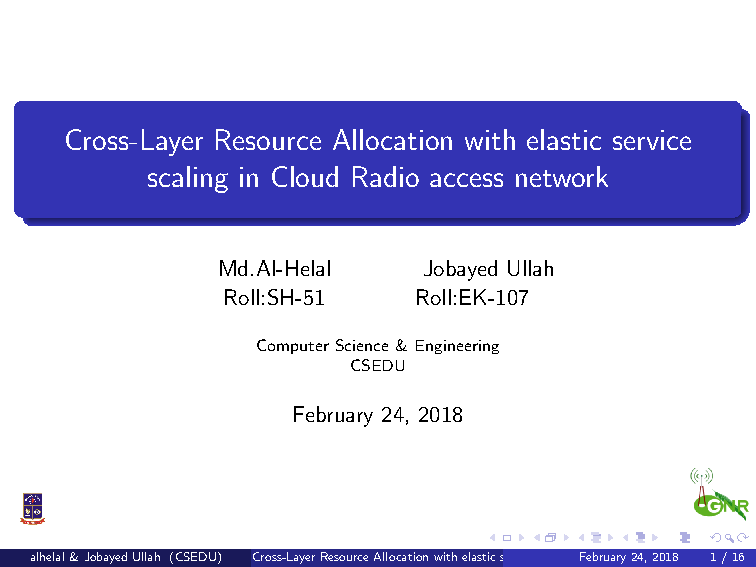
\includegraphics[width=1cm,height=1cm,keepaspectratio]{Image/GNR.png}%
  %\includegraphics[width=1cm,height=1cm,keepaspectratio]{example-image-a}%
}
\begin{document}
  \title{Resource  Allocation in Cloud Radio Access Network\\Presentation on 4th year project progress}
  \author[Md.Al-Helal \& Jobayed Ullah]{
  \parbox{2.5cm}{
\centering Md.Al-Helal\\Roll:SH-51}\hspace{3cm}
\parbox{2.5cm}{
{\centering Jobayed Ullah\\Roll:EK-107}}
\centering \vspace{1cm}\\Supervisor:\\Tamal Adhikary\\\scriptsize{Computer Science \& Engineering\\University of Dhaka}
}

\vspace{1cm}
%\institute[CSEDU]{Computer Science \& Engineering\\University of Dhaka}
\date{February 25, 2018}
\begin{frame}
  \maketitle
\end{frame}

\begin{frame}
\frametitle{Contents}
\tableofcontents
\end{frame}
\section{Background}

\begin{frame}
  \frametitle{Background}
  Traditional cellular, or Radio Access Networks (RAN), consisting of many standalone base stations (BTS) have some limitations-
  \begin{itemize}
    \item Each BTS is costly to build and operate.
    \item When more BTSs are added to a system to improve its capacity, interference among the BTSs is more severe as BTSs are closer to each other.
    \item Because users are mobile, the traffic of each BTS fluctuates (called 'tide effect'), and as a result, the average utilization rate of individual BTS is pretty low.
  \end{itemize}
\end{frame}
\section{Motivation}
\begin{frame}
  \frametitle{Motivation}
  \begin{itemize}
    \item As one of the promising evolution paths for future cellular network architecture, C-RAN has attracted high academic research interest.
    \item Meanwhile, because the native support of cooperative radio capability built into the C-RAN architecture, it also enables many advanced algorithms that were hard to implement in cellular networks, including Cooperative Multi-Point Transmission/Receiving, Network Coding, etc.
  \end{itemize}
\end{frame}
\section{Architechture Overview}
\begin{frame}
  \frametitle{Architechture Overview\cite{journals/corr/PengSLMW16}}
  \includegraphics[scale=0.3]{Image/cranArchiTrans.png}
  %\includegraphics[scale=0.3]{example-image-a}
\end{frame}
\begin{frame}
  \frametitle{Architechture Overview\cite{journals/twc/TangTQ15}}
  \includegraphics[scale=0.3]{Image/cranArchi3.png}
  %\includegraphics[scale=0.3]{example-image-a}
\end{frame}
\begin{frame}
  \frametitle{Architechture Overview\cite{conf/wiopt/AlabbasiC17}}
  \includegraphics[scale=0.3]{Image/cranArchi2.png}
  %\includegraphics[scale=0.3]{example-image-a}
\end{frame}
\begin{frame}
  \frametitle{Architechture Overview\cite{wiki:C-RAN}}
  \begin{itemize}
    \item Large scale centralized deployment: Allows hundreds of thousands of RRHs to connect to a centralized BBU pool.
    \item Native support to Collaborative Radio technologies: Any BBU can talk with any other BBU within the BBU pool with very high bandwidth (10Gbit/s and above) and low latency(10us level).
    \item  C-RAN BBU pool is built on open hardware, like x86/ARM CPU based servers. Real-time virtualization makes sure the resources in the pool can be allocated dynamically to base station software stacks, say 4G/3G/2G function modules from different vendors according to network load.
  \end{itemize}
\end{frame}
\section{Related Work}
\begin{frame}
  \frametitle{Related Work}
  In\cite{journals/twc/TangTQ15}, the authors propose and investigate a cross-layer resource allocation model for C-RAN to minimize the overall system power consumption in the BBU pool, fiber links and the remote radio heads (RRHs). They characterize the cross-layer resource allocation problem as a mixed-integer nonlinear programming (MINLP), which jointly considers elastic service scaling, RRH selection, and joint beamforming.
\end{frame}
\begin{frame}
  \frametitle{Related Work}
  In\cite{conf/wiopt/AlabbasiC17}, the authors analyze the delay performance of the end user’s request. They propose an end-to-end (from the central cloud to the end user) delay model (per user’s request) for different function split points. In that model, different delay requirements enforce different function splits, hence affect the system’s energy consumption. Therefore, they proposed several research directions to incorporate the proposed delay model in the problem of minimizing energy and bandwidth consumption in the network.
\end{frame}
\section{References}
\begin{frame}
  \frametitle{References}
  \printbibliography
%\bibliographystyle{plain} 
\end{frame}
\begin{frame}{\phantom{}}
 % \color{Brown}
  \color{Sepia}
  \centering \Huge\textbf{Thank You}
\end{frame}
\end{document}
